Object detection is one of the subtasks in the image domain.
It is an extension of the classical classification task, where additionally to the predicted class, the location of the object should be provided.
The location is normally given as a bounding box.
Various formats for the bounding box definition exist.
One common format is $bbox = (x1, y1, x2, y2)$, where $(x1, y1)$ being the coordinate of the upper left corner of the bounding box and $(x2, y2)$ the lower right corner TODO cite.
Another format, used in the coco dataset is $bbox = (x, y, w, h)$, where again $(x, y)$ define the upper left corner and $(w, h)$ the width and the height of the bounding box TOOD cite.
In this thesis the format of Redmon et al. \cite{yolov1} is used.
Which is defined as $bbox = (x_{rel}, y_{rel}, w_{rel}, h_{rel})$.
Here, $(x_{rel}, y_{rel})$ define the relative center of the bounding box and $(w_{rel}, h_{rel})$ the relative width and height of the bounding box.
Relative means that each coordinate is normalized over its corresponding axis.
E.g. $x_{rel}$ would be calculated through $x_{rel} = \frac{x_{abs}}{max_x}$, where $max_x$ being the image size in $x$ direction.
The advantages of this format are, that the definition of the bounding box becomes invariant to the image size.
One can resize the image without having to recalculate the bounding box, as it is the case with an absolute format.

\subsection{History of Object Detection}

\subsubsection{Sliding Window}
The simplest algorithm to detect objects in an image is the sliding window approach.
Before an object detection can be performed on an image, a classifier has to be trained.
This classifier is normally trained on image patches, where a patch has roughly the size of the objects it should classify.
The object detection phase starts by dividing the input image into patches.
Those patches are now fed to the classifier and when the predicted probability exceeds a predefined threshold the patch is considered to have an object in it.
It should be noted that classification accuracy can be improved by feeding overlapping patches into the classifier.
The resulting predicted bounding boxes now look like the image on the left side in fig. \ref{fig:nms_before_after}.
It contains multiple bounding boxes for the same object.
To have only one prediction per object, a \ac{NMS} algorithm is applied on the overlapping bounding boxes.
The results of the \ac{NMS} can be seen on the right side in fig. \ref{fig:nms_before_after}.

- TODO add tackle scale by using patches of different size

\begin{figure}
\begin{center}
    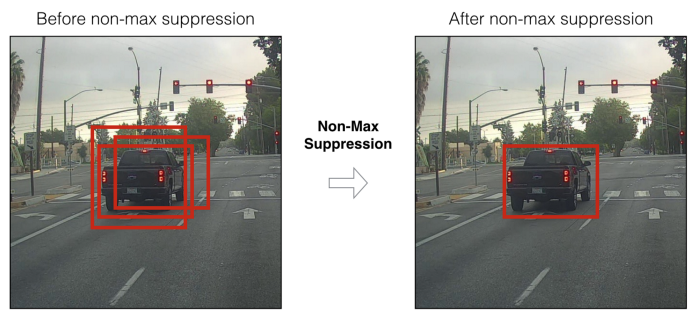
\includegraphics[width=16cm]{imgs/nms_before_after.png}
    \caption{Predicted bounding boxes before and after a non-maximum suppression was applied \cite{nms_before_after}}
    \label{fig:nms_before_after}
\end{center}
\end{figure}


\subsubsection{Regions with CNN Features (R-CNN)}
While the sliding window approach is effective, it is also highly inefficient, since all generated patches have to be processed in order to obtain the bounding boxes of the objects in an image.
\ac{R-CNN} by Girshick et al. \cite{rcnn} improves on that by using a region proposal algorithm to obtain probabel regions.
In contrast to brute forcing each possible region in an image this was a major improvement in performance.
In their work the selective search algorithm \cite{selective_search} was used to generate region proposals.
The selective search algorithm produces sub-segmentations of objects in an image, considering size, color, texture and shape based features, for the grouping of the regions.
How the algorithm performs and what kind of bounding boxes are produces can be seen in fig. \ref{fig:selective_search}.
The size of the regions is increased from left to right, additionally the proposed bounding boxes can be seen in the second row.
$2000$ of those proposed bounding boxes are now taken from different scales and warped into the input shape of the following \ac{CNN}, disregarding the size or aspect ratio of the proposed region.
Each region proposal is passed through the \ac{CNN} and yields a $4096$-dimensional feature vector.
The final step in the detection pipeline is comprised of feeding the $4096$-dimensional feature vector into $N + 1$ binary-\ac{SVMs}, where $N$ is the number of classes to predict plus one background class.

- TODO bbox regression fine tune

\begin{figure}
\begin{center}
    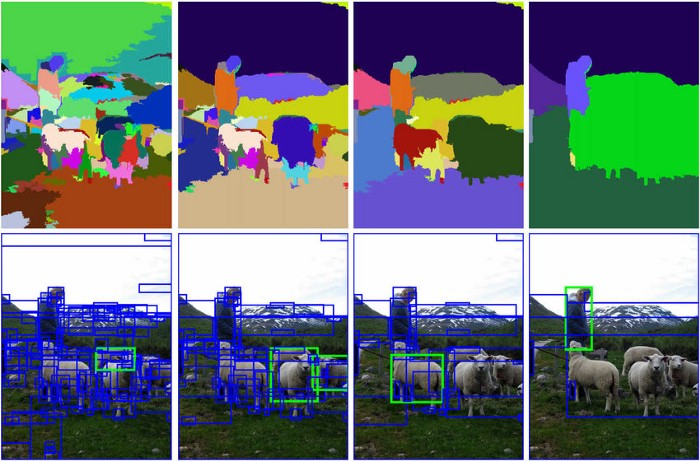
\includegraphics[width=13cm]{imgs/selective_search.png}
    \caption{Example of results obtained through the selective search algorithm with increasing region scale from left to right \cite{selective_search}}
    \label{fig:selective_search}
\end{center}
\end{figure}

\subsubsection{Fast R-CNN}

- faster through sharing computation

- spatial pyramid pooling to tackle arbitrary image sizes

- region proposal performed on feature maps

- joint multi task loss combining bbox reg and classification

\subsubsection{Faster R-CNN}



\subsubsection{Singleshot Detector}

\subsection{You Only Look Once}
